\section{Introduction}

SMRT inspects more than 1{,}000 buses, and each inspection includes measuring tyre tread depth by hand at several
points on every tyre. The UREX device replaces the hand gauge with a handheld optical head: a camera looks straight
down at the tread and a green line laser strikes the tread at an angle. Where the rubber is lower (inside a groove)
the laser line appears shifted in the image, and the size of the shift gives the depth. This is \emph{laser
triangulation}.

The software has one job: turn one greyscale image into a groove depth in millimetres, and a PASS / FAIL against the
1.6\,mm legal limit. The pipeline we had on 12 November (the \emph{baseline}) does this in three steps:
(1) find the laser line with a Steger ridge detector, (2) fit the tread surface and read how far the line drops
inside each groove, (3) convert pixels to millimetres with a calibration. It works on good photos, but it also
reports a depth on most \emph{bad} photos, and it has never been tested against known answers.

This report asks a practical question: \textbf{which algorithms actually make the software more robust, and by how
much?} To answer it we built a simulator of the printed holder, a fixed benchmark with exact ground truth, and then
tried ten families of algorithms, each on its own git branch, all scored by the same harness on the same frames and
on the 86 real photos taken between 8 and 30 October.

\paragraph{Contributions.}
\begin{itemize}
\item A ray-traced simulator of the Rev\,A holder on a tyre, with exact truth for the laser line and every groove
      (Section~\ref{sec:sim}).
\item A benchmark of five simulated test sets plus the real photos, and a scorer that rewards an algorithm for
      saying ``retake the photo'' instead of guessing (Section~\ref{sec:bench}).
\item A like-for-like evaluation of ten algorithm families: sub-pixel peak detectors, dynamic-programming line
      tracking, a small U-Net, a candidate classifier, a robust depth stage, calibration models, a quality gate,
      laser on/off subtraction, an end-to-end network, and a combined stack (Sections~\ref{sec:algos}--\ref{sec:stack}).
\item An independent audit of the numbers (Section~\ref{sec:audit}), and an honest list of what the simulator and the
      real photos can and cannot tell us (Section~\ref{sec:validity}).
\end{itemize}

\section{The device and the measurement}\label{sec:device}

Figure~\ref{fig:geometry} shows the geometry of the printed holder. The holder's feet rest on the tread, so the
camera height and the laser angle are fixed. The numbers used throughout are in Table~\ref{tab:device}.

\begin{figure}[H]
\centering
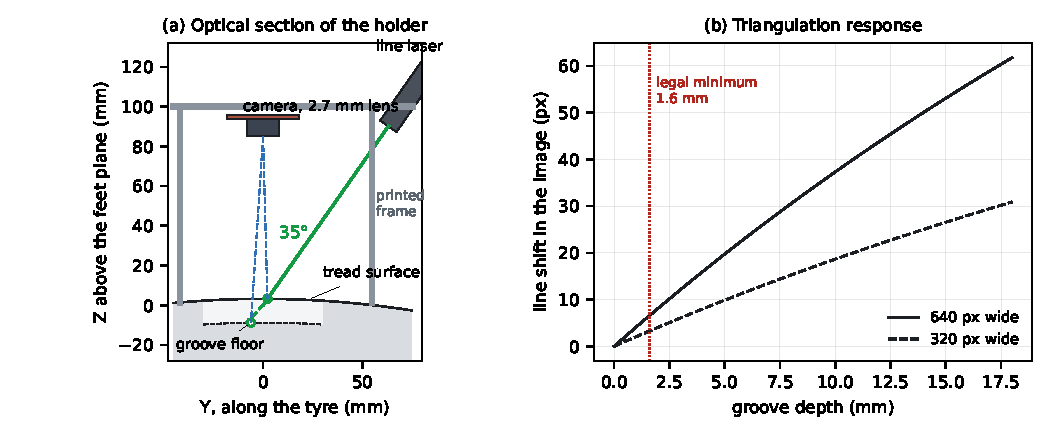
\includegraphics[width=0.86\linewidth]{figs/fig_geometry.pdf}
\caption{Side view of the holder on a tyre. The camera looks straight down; the laser sheet arrives at
$35^\circ$. A groove floor lies lower than the tread, so the laser meets it further along, and the camera sees the
line shifted.}
\label{fig:geometry}
\end{figure}

\begin{table}[H]
\centering\small
\caption{Device constants (holder Rev\,A, OV5640 camera with a 2.7\,mm lens).}\label{tab:device}
\begin{tabular}{@{}lll@{}}
\toprule
Quantity & Value & Comment \\
\midrule
Camera height above the feet plane & 85\,mm & lens front, looking straight down \\
Focal length & 2.7\,mm (235\,px at 320\,px image width) & horizontal field of view $68^\circ$ \\
Laser angle $\theta$ & $35^\circ$ from vertical & $110^\circ$ fan across the tread \\
Tyre radius / crown height & 480\,mm / 3.2\,mm above the feet plane & bus tyre between the feet \\
Image used by the algorithms & $320\times240$ greyscale & down-sampled; real photos are $240\times320$ \\
Legal limit & 1.6\,mm & PASS only if every groove is deeper \\
\bottomrule
\end{tabular}
\end{table}

\paragraph{How a depth becomes a pixel shift.} Let $H$ be the distance from the lens to the tread surface
(about 82\,mm) and $f$ the focal length in pixels. A groove of depth $d$ moves the laser spot sideways by
$d\tan\theta$ on the tyre and puts it $d$ further from the camera, so the line moves in the image by
\begin{equation}
\Delta v \;=\; \frac{f\, d \tan\theta}{H + d}
\qquad\Longrightarrow\qquad
d \;=\; \frac{H\,\Delta v}{f\tan\theta - \Delta v}.
\label{eq:tri}
\end{equation}
With our numbers this is about \textbf{2.1\,px of shift per millimetre of depth}, and about 2.9\,px per millimetre
across the tread. Two consequences follow, and they explain most of this report:
\begin{itemize}
\item An error of only 0.2\,px in locating the line is already 0.1\,mm of depth. Sub-pixel accuracy matters.
\item One wrong decision about \emph{which bright thing is the laser} (a glint, a wet patch, the edge of a thick
      saturated line) is an error of many millimetres. Robustness matters more.
\end{itemize}
In practice we do not use Eq.~\eqref{eq:tri} directly. A calibration (Section~\ref{sec:calib}) maps each image
position to a height, which also absorbs lens distortion and assembly tolerances.

\section{Method: simulator, benchmark and scorer}

\subsection{Simulator}\label{sec:sim}

Real photos have no ground truth: nobody measured those grooves with a gauge. So we wrote a simulator,
\texttt{research/sim/holder\_sim.py}, that renders what the camera in the holder would see. It builds a tyre
surface (radius 480\,mm, a gentle crown, circumferential grooves with sloped walls and optional rounded floors),
traces 2{,}400 laser rays to the first surface they hit, checks that the camera can see each hit, and renders the
line with realistic blur, sensor noise, lens distortion and JPEG compression. Because the scene is known, every
frame comes with the exact sub-pixel laser line and the exact depth of every groove, plus a laser-off frame of the
same scene.

The simulator can also make conditions worse on purpose: rocking of the holder, sunlight, wet glints, stones in
grooves, zig-zag grooves, mud that hides part of the line, paint, a dim or a saturated laser. Figure~\ref{fig:simreal}
compares simulated frames with real photos.

\begin{figure}[H]
\centering
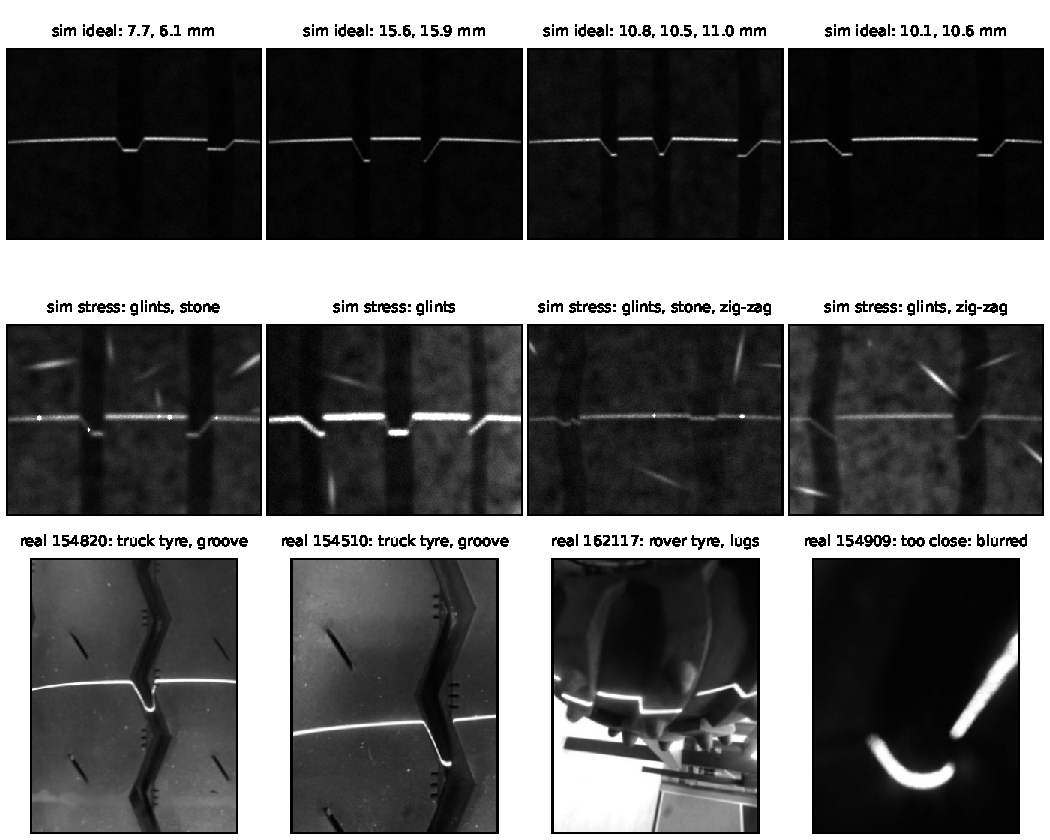
\includegraphics[width=\linewidth]{figs/fig_sim_vs_real.pdf}
\caption{Simulated frames (holder locked in place) next to real photos (hand-held, October). The simulated ``ideal''
line is thin and level; real lines are thicker, often saturated, and can sit anywhere in the frame.}
\label{fig:simreal}
\end{figure}

\subsection{Test sets}\label{sec:bench}

\begin{table}[H]
\centering\small
\caption{The benchmark. Algorithms may train or tune only on \texttt{train}; all other sets are for testing.}\label{tab:sets}
\begin{tabularx}{\linewidth}{@{}llX@{}}
\toprule
Set & Frames & What it represents \\
\midrule
\texttt{ideal} & 150 & Holder locked on a clean tyre in shade: the conditions the holder is designed to create. \\
\texttt{stress} & 200 & Rocking $\pm1^\circ$, sunlight, wet glints, stones, zig-zag grooves, mud gaps, paint, blur, dim or saturated laser. \\
\texttt{legal} & 150 & Worn tyres, grooves 0.6--3.5\,mm: the PASS/FAIL boundary at 1.6\,mm. \\
\texttt{shifted} & 150 & Three \emph{other} holder units (laser at $33^\circ$, $36^\circ$, $37^\circ$; small roll and height errors), each with its own calibration. Tests whether a method survives a different unit. \\
\texttt{handheld} & 150 & Built to look like the real photos: thick saturated line, line anywhere in the frame, clutter. Scored in pixels. \\
\texttt{train} & 1{,}200 & Mixed conditions, different random seed. Training only. \\
\texttt{calib} & 15 & Flat plate at 15 known heights from $+6$ to $-22$\,mm. \\
\midrule
real photos & 86 & Hand-held photos, 8--30 October. A person would measure 19 of them. Six truck-tyre frames have a reference groove depth in pixels. \\
\bottomrule
\end{tabularx}
\end{table}

\subsection{What is scored}

Every algorithm is a Python module with the same interface: image in, list of grooves out (plus, optionally, the
laser line it found and a number saying whether the frame is usable). The scorer reports:

\begin{itemize}
\item \textbf{Coverage}: share of frames the algorithm answers. An algorithm may \emph{abstain} (``retake'').
\item \textbf{Depth MAE, median, P95}: mean, median and 95th-percentile absolute depth error over grooves that were
      found, in mm. The mean is dominated by a few huge errors; the median shows the typical case.
\item \textbf{Gross}: share of grooves wrong by more than 1\,mm (3\,px on \texttt{handheld}).
\item \textbf{Miss}: measurable grooves that were not reported. \textbf{False}: reported grooves per frame where
      there is none.
\item \textbf{Verdict}: PASS/FAIL accuracy at 1.6\,mm over answered frames. \textbf{F.pass}: unsafe mistakes (the
      tyre is illegal and the algorithm says PASS), counted over \emph{all} frames.
\item \textbf{CPU ms}: processor time per frame on one laptop-class core.
\end{itemize}

For real photos there is no ground truth, so the scorer reports agreement instead: agreement of the line with a
reference line on the six truck-tyre frames, the difference from the reference depth in pixels, how many of the
19 good photos are kept, and on how many of the 67 bad photos a depth is (wrongly) reported.

\caution{The real-photo references were produced by the baseline pipeline and then checked by eye. The baseline
therefore scores ``perfect'' on them by construction. On real photos, read the numbers as \emph{agreement with the
baseline on frames where the baseline looked right}, not as accuracy.}
